\chapter{Análisis funcional} \label{cap:analisis}

\section{Introducción}

Este capítulo ofrece una visión general del sistema, comenzando con una introducción preliminar, seguida de la identificación de los actores involucrados. A continuación, se detallarán los casos de uso mediante un diagrama contextual general, para después desglosar y afinar cada caso de uso que compone la aplicación. Finalmente, este capítulo concluirá con la validación de los casos de uso en relación con los requisitos funcionales previamente descritos.

Un caso de uso describe una secuencia de acciones realizadas por el sistema en respuesta a las interacciones de un actor, especificando el comportamiento del sistema o de una parte del mismo.

Un diagrama de casos de uso representa visualmente un conjunto de casos de uso, las relaciones entre ellos y los actores involucrados. Este diagrama se utiliza para modelar la vista estática de un sistema, permitiendo visualizar su comportamiento externo y, de esta manera, identificar qué debe hacer el sistema independientemente de cómo se implementará.

Los casos de uso del sistema se especificarán según los siguientes aspectos:

\begin{itemize}
    \item \textbf{Nombre}: denominación completa y codificación del diagrama de casos de uso.
    \item \textbf{Actor}: usuario participante en el diagrama.
    \item \textbf{Descripción}: breve explicación del diagrama en su conjunto.
    \item \textbf{Casos de uso}: lista y breve descripción de los casos de uso presentes en el diagrama.
    \item \textbf{Flujo de eventos principal}: enumeración de los pasos que debe seguir el actor para lograr el objetivo del caso de uso.
    \item \textbf{Flujo de eventos alternativo}: pasos a seguir en caso de que el actor no pueda alcanzar el objetivo principal del caso de uso.
\end{itemize}

\section{Actores del Sistema}

Como se mencionó en el capítulo anterior, el sistema cuenta con un único tipo de actor final, que incluye tanto a \textit{profesores} como a \textit{alumnos} que utilizan el software para realizar análisis de gramáticas de contexto libre.

Por lo tanto, la especificación de los casos de uso que se presenta a continuación se centra exclusivamente en el actor del sistema, denominado \textbf{Usuario}.


\section{Especificación de casos de uso}

En esta sección, se procederá a especificar cada caso de uso detalladamente, siguiendo el esquema previamente mencionado. Se iniciará con la presentación de un diagrama de casos de uso de contexto, que proporcionará una visión general de la interacción entre el usuario y el sistema. Luego, cada caso de uso será refinado individualmente para ofrecer una comprensión profunda de las funcionalidades y comportamientos esperados del sistema.


\begin{figure}[H]
    \begin{center} 
        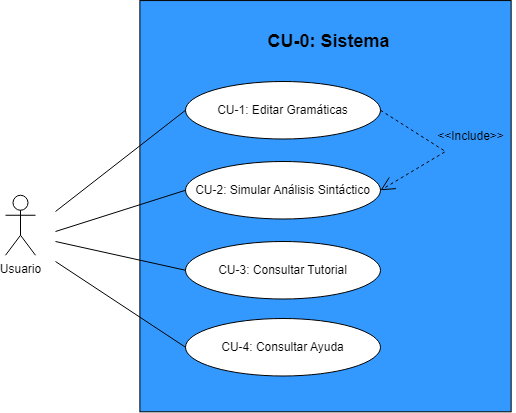
\includegraphics[scale=0.55]{figuras/Cap7/CU0.png}
        \caption{Diagrama de contexto del Sistema}
        \label{fig:diagramaContexto}
    \end{center}
\end{figure}

\subsection{Diagrama de contexto: CU-0. Sistema}

La figura \ref{fig:diagramaContexto}  presenta el diagrama de contexto del sistema, en el cual se identifican los cuatro casos de uso principales que conforman la aplicación. Estos casos de uso son:
\begin{itemize}
    \item \textbf{CU-1. Editar gramática}: corresponde al módulo para la \textit{edición de gramáticas}.
    \item \textbf{CU-2. Simular análisis sintáctico descendente predictivo}: se refiere al módulo que \textit{simula el analizador sintáctico descendente predictivo utilizando gramáticas de contexto libre}.    
    \item \textbf{CU-3. Consultar tutorial}: relacionado con el módulo del \textit{tutorial}.    
    \item \textbf{CU-4. Consultar ayuda}: está relacionado con el módulo de la \textit{ayuda}.
\end{itemize}



La especificación del caso de uso CU-0. Sistema se presenta en la tabla \ref{tabla71}.

\begin{longtable}[htp]{|>{\columncolor[rgb]{0.63,0.79,0.95}}m{6cm} | m{8.5cm} |}
    \caption{Caso de uso: CU-0. Sistema}
    \endfirsthead
    \multicolumn{2}{c}{{\tablename\ \thetable{} -- continua de la página anterior}} \\
    \endhead
    \hline \multicolumn{2}{|r|}{{Continúa en la página siguiente}} \\ \hline
    \endfoot

    \hline
    \endlastfoot

    \hline
    \textbf{Nombre} & \textbf{CU-0. Sistema} (diagrama de contexto).\newline \textbf{Nivel}: 0  \\ 
    \hline
    \textbf{Descripción} &  Proporciona al usuario una visión general de todos los subsistemas que componen la aplicación, registrando todas las interacciones posibles del usuario con estos. \\ \hline                       
    \textbf{Actores} & Usuario \\ \hline

    \textbf{Casos de uso} & \begin{enumerate}
        \item \textbf{CU-1. Editar Gramáticas}: este subsistema se encarga de la edición de gramáticas de contexto libre.                                   
        \item \textbf{CU-2. Simular análisis sintáctico descendente predictivo}: este subsistema se dedica a la simulación del analizador sintáctico descendente predictivo utilizando gramáticas de contexto libre.
        \item \textbf{CU-3. Consultar Tutorial}: proporciona acceso al tutorial de la aplicación.
        \item \textbf{CU-4. Consultar Ayuda}: permite acceder a la ayuda de la aplicación.
    \end{enumerate} 
    \\ \hline
    \textbf{Flujo de eventos principal} & \begin{enumerate}
        \item El usuario inicia sesión en el Sistema.
        \item Se presentan todas las opciones disponibles al usuario.
        \item El usuario selecciona una opción del Sistema.
        \item El Sistema procesa la selección del usuario.
        \item Se proporciona retroalimentación al usuario sobre la selección realizada.
        \item El usuario interactúa con el subsistema seleccionado (por ejemplo, edición de gramáticas, simulación, consulta de tutoriales o ayuda).
        \item El usuario puede guardar su progreso y retornar al menú principal en cualquier momento.
    \end{enumerate} \\ \hline
    \textbf{Flujo de eventos alternativo} & \begin{enumerate}
        \item Ocurre un error durante la inicialización del Sistema.
        \item Se notifica al usuario sobre el error.
        \item El Sistema sugiere posibles soluciones o pasos a seguir para resolver el problema.
        \item Si el error persiste, el Sistema guarda cualquier progreso no guardado previamente y cierra la aplicación de manera segura.
        \item El usuario es redirigido a una página de soporte técnico para obtener asistencia adicional.
    \end{enumerate} 
    \label{tabla71}
\end{longtable}

A continuación, se procederá a detallar todos los casos de uso que conforman las funcionalidades del simulador. Este análisis detallado se realizará de manera sistemática, abordando cada caso de uso general identificado en el diagrama de contexto (figura \ref{fig:diagramaContexto}): CU-1, CU-2, CU-3 y CU-4.


\subsection{CU-1. Editar Gramáticas}

Este caso de uso representa la edición de gramáticas de contexto libre en el sistema. 

  \begin{figure}[H]
       \begin{center} 
 	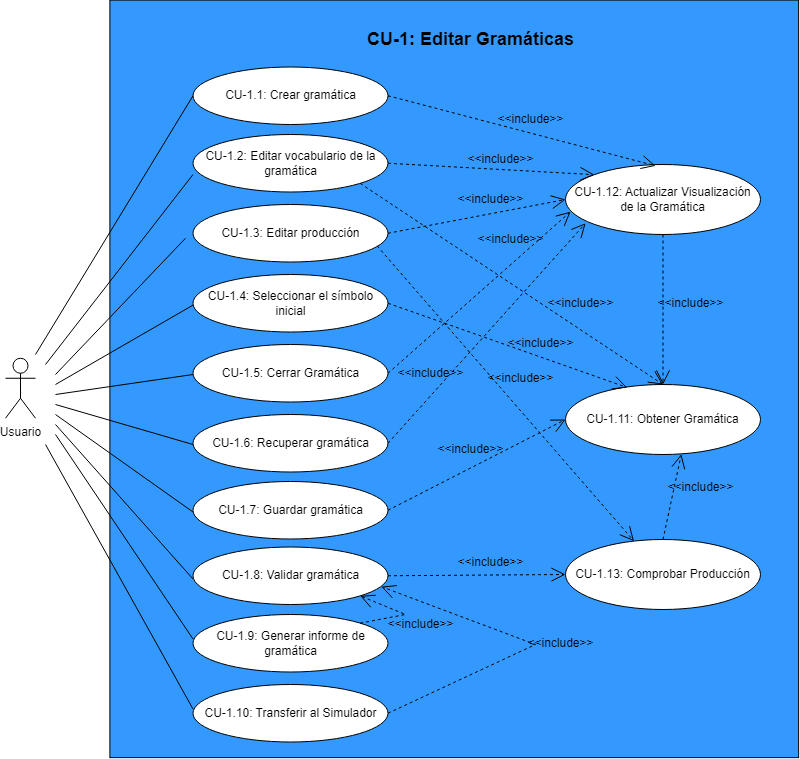
\includegraphics[scale=0.55]{figuras/Cap7/CU1.png}
 	\caption{CU-1: Editar Gramáticas}
 	\label{fig:CU1_EdicionDeGramatica}
      \end{center}
   \end{figure}

La figura \ref{fig:CU1_EdicionDeGramatica} muestra la representación gráfica de este caso de uso, que está formado por los siguientes sub-casos de uso:

 \begin{itemize}
  \item \textbf{CU-1.1. Crear gramática}.
  \item \textbf{CU-1.2. Editar vocabulario de la gramática}.
  \item \textbf{CU-1.3. Editar producción}.
  \item \textbf{CU-1.4. Seleccionar el símbolo inicial}.
  \item \textbf{CU-1.5. Cerrar gramática}.
  \item \textbf{CU-1.6. Recuperar gramática}.
  \item \textbf{CU-1.7. Guardar gramática}.
  \item \textbf{CU-1.8. Validar gramática}.
  \item \textbf{CU-1.9. Generar informe de gramática}.
  \item \textbf{CU-1.10. Transferir al simulador}.
  \item \textbf{CU-1.11. Obtener gramática}.
  \item \textbf{CU-1.12. Actualizar visualización de la gramática}.
  \item \textbf{CU-1.13. Comprobar producción}.
 \end{itemize}


 \begin{longtable}[H]{|>{\columncolor[rgb]{0.63,0.79,0.95}}p{6cm} | p{8.5cm} |}
    \caption{Caso de uso: CU-1. Edición de gramáticas}
    \label{tablaCU1} \\
    \hline
    \textbf{Nombre} & \textbf{CU-1. Editar Gramáticas} \newline \textbf{Nivel}: 1 \\
    \hline
    \textbf{Descripción} & Permite al usuario la creación y edición de gramáticas de contexto libre. \\
    \hline
    \textbf{Actores} & Usuario \\
    \hline
    \textbf{Casos de uso} & 
    \begin{enumerate}
        \item \textbf{CU-1.1. Crear gramática}: permite \textit{crear} una gramática a partir de una producción inicial.
        \item \textbf{CU-1.2. Editar vocabulario de la gramática}: permite \textit{editar} el vocabulario de símbolos ($V_{N}, V_{T}$) de la gramática.
        \item \textbf{CU-1.3. Editar producción}: permite la \textit{edición} de producciones de la gramática.
        \item \textbf{CU-1.4. Seleccionar el símbolo inicial}: permite la \textit{selección} del símbolo inicial de la gramática.
        \item \textbf{CU-1.5. Cerrar gramática}: \textit{cierra} una gramática abierta en el editor.
        \item \textbf{CU-1.6. Recuperar gramática}: \textit{carga} una gramática almacenada en un fichero.
        \item \textbf{CU-1.7. Guardar gramática}: \textit{almacena} una gramática en un fichero.
        \item \textbf{CU-1.8. Validar gramática}: \textit{valida} una gramática de contexto libre.
        \item \textbf{CU-1.9. Generar informe}: \textit{genera} un informe de una gramática de contexto libre.
        \item \textbf{CU-1.10. Transferir al simulador}: \textit{transfiere} una gramática de contexto libre al simulador para simular el análisis sintáctico.
        \item \textbf{CU-1.11. Obtener gramática}: \textit{obtiene} el vocabulario de símbolos ($V_{N}, V_{T}$) así como las producciones de la gramática.
        \item \textbf{CU-1.12. Actualizar visualización de la gramática}: \textit{actualiza} la visualización de la gramática en la interfaz del simulador para permitir al usuario visualizarla a medida que realiza modificaciones en la misma.
        \item \textbf{CU-1.13. Comprobar producción}: \textit{comprueba} si una regla gramatical o producción es correcta o no.
    \end{enumerate} \\
    \hline
    \textbf{Flujo de eventos principal} & 
    \begin{enumerate}
        \item El usuario accede al Sistema.
        \item Se presentan todas las opciones disponibles al usuario.
        \item El usuario selecciona una de las opciones del Sistema.
        \item El Sistema ejecuta la acción correspondiente a la opción seleccionada.
        \item El Sistema proporciona retroalimentación al usuario sobre la acción realizada.
        \item El usuario puede guardar su progreso y retornar al menú principal en cualquier momento.
    \end{enumerate} \\
    \hline
    \textbf{Flujo de eventos alternativo} & 
    \begin{enumerate}
        \item Ocurre un error durante la inicialización del Sistema.
        \item Se notifica al usuario sobre el error.
        \item El Sistema sugiere posibles soluciones o pasos a seguir para resolver el problema.
        \item Si el error persiste, el Sistema guarda cualquier progreso no guardado previamente y cierra la aplicación de manera segura.
        \item El usuario es redirigido a una página de soporte técnico para obtener asistencia adicional.
    \end{enumerate} \\
    \hline
    \textbf{Flujo de eventos alternativo adicional} & La acción representada por el caso de uso CU-1.12 se lleva a cabo de forma continua, sin que lo solicite el usuario. Además, esta acción se ejecuta cada vez que el usuario modifica la gramática utilizando alguno de los casos de uso que implican este sub-caso de uso. \\
    \hline
\end{longtable}


 En las siguientes secciones, se refinará cada uno de los sub-casos de uso que componen el caso de uso CU-1.

\subsubsection{CU-1.1. Crear gramática}

Este caso de uso describe el proceso de creación de una gramática de contexto libre. La figura \ref{fig:CU1.1_CrearGramatica} muestra la representación gráfica del caso de uso, mientras que la tabla \ref{tabla73} presenta su descripción tabular.

 \begin{figure}[H]
       \begin{center} 
 	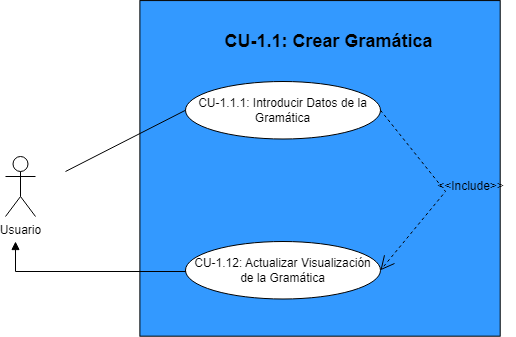
\includegraphics[scale=0.55]{figuras/Cap7/CU11.png}
 	\caption{CU-1.1: Crear gramática}
 	\label{fig:CU1.1_CrearGramatica}
       \end{center}
   \end{figure}

 \begin{longtable}[H]{|>{\columncolor[rgb]{0.63,0.79,0.95}}m{6cm} | m{8.5cm} |}
 \caption{Caso de uso: CU-1.1 Crear gramática} \\
 \endfirsthead
 \multicolumn{2}{c}
 {{ \tablename\ \thetable{} -- continúa de la página anterior}} \\
 \endhead
 \hline \multicolumn{2}{|r|}{{continúa en la página siguiente}} \\ \hline
 \endfoot
 \hline
 \endlastfoot
  \hline
  \textbf{Nombre} & \textbf{CU-1.1 Crear gramática}.\newline \textbf{Nivel}: 2  \\ \hline
  \textbf{Descripción} &  Permite al usuario crear gramáticas de contexto libre. \\ \hline                       
  \textbf{Actores} & Usuario \\ \hline
   \textbf{Casos de uso} & \begin{enumerate}
   \item \textbf{CU-1.1.1 Introducir datos de la gramática}: permite que el usuario \textit{introduzca} los datos de una gramática de contexto libre.
   \item \textbf{CU-1.1.2 Actualizar visualización de la gramática}: \textit{actualiza} la visualización de la gramática en la interfaz del simulador. 
   \end{enumerate} \\ \hline
   \textbf{Flujo de eventos principal} & 
   \begin{enumerate}
   \item El usuario introduce el nombre de la gramática y una descripción de la misma.
    \item Se crea la gramática y se actualiza la visualización en la interfaz.
    \item El usuario recibe una confirmación de la creación exitosa de la gramática.
   \end{enumerate} \\ \hline
   \textbf{Flujo de eventos alternativo} & 
   \begin{enumerate}
        \item Si en el paso 2 se detecta algún error durante la actualización de la visualización:
        \begin{enumerate}
        \item Se informa al usuario del error producido.
        \item El sistema proporciona posibles soluciones o pasos a seguir.
        \end{enumerate}
    \end{enumerate} 
   \label{tabla73}
 \end{longtable}

El caso de uso \textit{CU-1.1.1 Introducir datos de la gramática} no requiere un refinamiento adicional debido a su simplicidad. Este caso de uso se encarga de solicitar al usuario el nombre y la descripción de la gramática, excluyendo símbolos y producciones, para posteriormente incorporarlos en la definición de la gramática.

\subsubsection{CU-1.2. Editar vocabulario de la gramática}

Este caso de uso describe el proceso de edición del vocabulario de la gramática, incluyendo tanto los símbolos terminales como los no terminales. La figura \ref{fig:CU1.2} muestra la representación gráfica del caso de uso, mientras que la tabla \ref{tabla74} presenta su descripción tabular.

  \begin{figure}[H]
       \begin{center} 
 	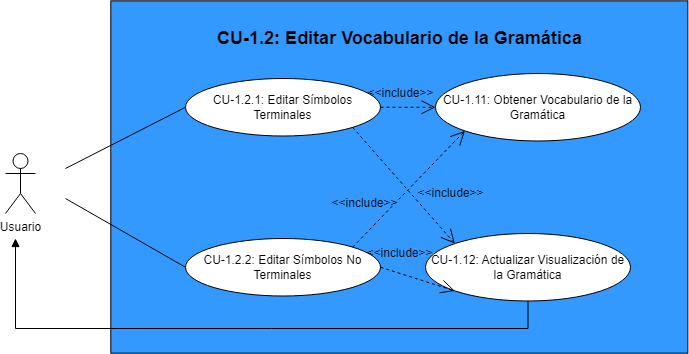
\includegraphics[scale=0.55]{figuras/Cap7/CU12.png}
 	\caption{CU-1.2: Editar vocabulario de la gramática}
 	\label{fig:CU1.2}
       \end{center}
   \end{figure}

 \begin{longtable}[H]{|>{\columncolor[rgb]{0.63,0.79,0.95}}m{6cm} | m{8.5cm} |}
 \caption{Caso de uso: CU-1.2 Editar vocabulario de la gramática} \\
 \endfirsthead
 \multicolumn{2}{c}
 {{ \tablename\ \thetable{} -- continúa de la página anterior}} \\
 \endhead
 \hline \multicolumn{2}{|r|}{{continúa en la página siguiente}} \\ \hline
 \endfoot
 \hline
 \endlastfoot
 \hline
 \textbf{Nombre} & \textbf{CU-1.2 Editar vocabulario de la gramática}.\newline \textbf{Nivel}: 2  \\ \hline
 \textbf{Descripción} &  Permite al usuario editar el vocabulario ($V_{N}, V_{T}$) de la gramática. \\ \hline
 \textbf{Actores} & Usuario \\ \hline
  \textbf{Casos de uso} & 
     \begin{enumerate}
     \item \textbf{CU-1.2.1. Editar símbolos terminales}: permite que el usuario \textit{introduzca o modifique} el conjunto de símbolos terminales de la gramática.
     \item \textbf{CU-1.2.2. Editar símbolos no terminales}: permite que el usuario \textit{introduzca o modifique} el conjunto de símbolos no terminales de la gramática. 
     \item \textbf{CU-1.11. Obtener gramática}: \textit{obtiene} el vocabulario de símbolos ($V_{N}, V_{T}$) así como las producciones de la gramática.
     \item \textbf{CU-1.12. Actualizar vi\-sua\-li\-za\-ción de la gramática}: \textit{actualiza} la visualización de la gramática en la interfaz del simulador.
     \end{enumerate} \\ \hline
  \textbf{Flujo de eventos principal} & 
     \begin{enumerate}
     \item El usuario elige entre alguna de las opciones disponibles:
         \begin{enumerate}
         \item Introducir el conjunto de símbolos terminales de la   gramática y se comprueba si son correctos.
         \item Introducir el conjunto de símbolos no terminales de la  gramática y se comprueba si son correctos.     
         \end{enumerate} 
     \end{enumerate} \\ \hline                     
  \textbf{Flujo de eventos alternativo} & Si durante la opción o función 1, se detecta que alguno de los símbolos terminales introducido no es co\-rrec\-to:
     \begin{enumerate}
     \item Se informa al usuario del error producido.
     \item Se pide al usuario que reintroduzca el símbolo terminal que produjo el error.
     \end{enumerate}\\ \hline              
   \textbf{Flujo de eventos alternativo} & Si durante la opción o función 2, se detecta que alguno de los símbolos no terminales introducido no es co\-rrec\-to:
     \begin{enumerate}
     \item Se informa al usuario del error producido.
     \item Se pide al usuario que reintroduzca el símbolo no terminal que produjo el error.
     \end{enumerate}         
   \label{tabla74}
 \end{longtable}

 Los casos de uso \textit{CU-1.2.1 Editar símbolos terminales} y \textit{CU-1.2.2 Editar símbolos no terminales} no se refinarán más, puesto que son casos de uso bastante sencillos y que pueden ser fácilmente traducidos a una implementación posterior sin necesidad de ser refinados.

 El caso de uso CU-1.2.1 mostrará al usuario una ventana para \textit{introducir} o \textit{modificar} (en el caso de que ya los haya introducido) todos los símbolos terminales de la gramática, mientras que el caso de uso CU-1.2.2 permitirá modificar los no terminales.

 \subsubsection{CU-1.3. Editar producción}

 Este caso de uso representa la edición de una producción de una gramática. En la figura \ref{fig:CU13} se muestra la representación gráfica del caso de uso y en la tabla \ref{tabla75} se muestra su representación tabular.

 \begin{figure}[H]
       \begin{center} 
 	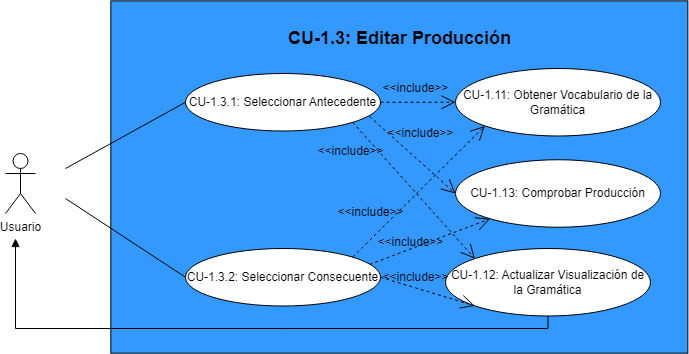
\includegraphics[scale=0.55]{figuras/Cap7/CU13.png}
 	\caption{CU-1.3: Editar producción}
 	\label{fig:CU13}
       \end{center}
 \end{figure}


 \begin{longtable}[H]{|>{\columncolor[rgb]{0.63,0.79,0.95}}m{6cm} | m{8.5cm} |}
 \caption{Caso de uso: CU-1.3: Editar producción} \\
 \endfirsthead
 \multicolumn{2}{c}
 {{ \tablename\ \thetable{} -- continúa de la página anterior}} \\
 \endhead
 \hline \multicolumn{2}{|r|}{{continúa en la página siguiente}} \\ \hline
 \endfoot
 \hline
 \endlastfoot

  \hline
  \textbf{Nombre} & \textbf{CU-1.3 Editar producción}.\newline \textbf{Nivel}: 2  \\ \hline
  \textbf{Descripción} & Permite al usuario editar una producción de la gramática de contexto libre.\\ \hline
  \textbf{Actores} & Usuario \\ \hline
  \textbf{Casos de uso} & 
     \begin{enumerate}
     \item \textbf{CU-1.3.1 Seleccionar antecedente}: permite que el usuario \textit{modifique}  el antecedente de una producción.
     \item \textbf{CU-1.3.2 Seleccionar consecuente}: permite que el usuario \textit{modifique}  el consecuente de una producción.
     \item \textbf{CU-1.11. Obtener gramática}: \textit{obtiene} el vocabulario de símbolos ($V_{N}, V_{T}$) así como las producciones de la gramática.
     \item \textbf{CU-1.12. Actualizar vi\-sua\-li\-za\-ción de la gramática}: \textit{actualiza} la visualización de la gramática en la interfaz del simulador.
     \item \textbf{CU-1.13 Comprobar producción}: \textit{comprueba} si una producción es correcta.
     \end{enumerate} \\ \hline
      \textbf{Flujo de eventos principal} & 
         \begin{enumerate}
         \item El usuario \textit{selecciona} el antecedente o el consecuente (o  ambos) de la producción que desea crear o modificar (en caso de que en CU-1 el usuario hubiera seleccionado alguna producción que ya existía).
         \item El usuario \textit{modifica} el antecedente o el consecuente (o ambos).
         \item Se \textit{comprueba} si la producción modificada es correcta.
         \end{enumerate} \\ \hline
  \textbf{Flujo de eventos alternativo} & Si no existe ningún símbolo en el vocabulario de la gramática (o solamente existe uno de los conjuntos de símbolos: terminales o no terminales) o bien alguno de los símbolos posee un error, se procede como sigue:
     \begin{enumerate}
     \item Se \textit{informa} al usuario del evento y se le pide que introduzca o modifique el conjunto de símbolos de la gramática.
     \end{enumerate} \\ \hline          
  \textbf{Flujo de eventos alternativo} & Si se produce algún fallo durante el paso 2, se procede como sigue:
     \begin{enumerate}
     \item Se \textit{informa} al usuario del error producido.
     \item Se \textit{deshacen} los cambios re\-a\-li\-zados por el usuario en la producción.
     \end{enumerate} \\ \hline              
   \textbf{Flujo de eventos alternativo} & Si se comprueba la producción resultante y esta no es correcta, se procede como sigue:
   \begin{enumerate}
   \item Se \textit{informa} al usuario del error (diciendo además si está en el antecedente,  en el consecuente o en ambos) y el motivo del mismo.
   \item Se \textit{pide} al usuario que corrija el e\-rror.              \end{enumerate}
   \label{tabla75}
 \end{longtable}

 Los casos de uso \textit{CU-1.3.1 Seleccionar antecedente} y \textit{CU-1.3.2 Seleccionar consecuente} no se refinarán más, puesto que son casos de uso bastante sencillos y que pueden ser fácilmente traducidos a una implementación posterior sin necesidad de ser refinados.

 El caso de uso CU-1.3.1 mostrará un diálogo al usuario que le permita seleccionar el antecedente de la producción de entre los símbolos no terminales que introdujo (mediante el caso de uso 1.2).

 El caso de uso CU-1.3.2, por su parte, permitirá al usuario modificar el consecuente de la producción (re\-a\-li\-zando acciones análogas a la del caso de uso 1.3.1).

 \subsubsection{CU-1.4. Seleccionar el símbolo inicial}

 Este caso de uso representa la selección del símbolo inicial de la gramática. En la figura \ref{fig:CU14} se muestra la representación gráfica del caso de uso y en la  tabla \ref{tabla76} se muestra su representación tabular.

   \begin{figure}[H]
       \begin{center} 
 	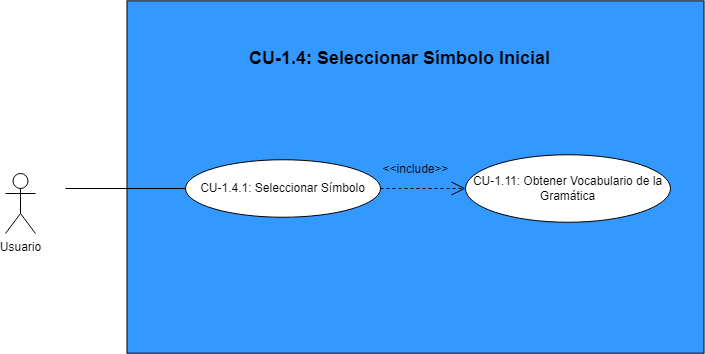
\includegraphics[scale=0.55]{figuras/Cap7/CU14.png}
 	\caption{CU-1.4: Seleccionar el símbolo inicial}
 	\label{fig:CU14}
       \end{center}
   \end{figure}


 \begin{longtable}[H]{|>{\columncolor[rgb]{0.63,0.79,0.95}}m{6cm} | m{8.5cm} |}
 \caption{Caso de uso: CU-1.4 Seleccionar el símbolo inicial} \\
 \endfirsthead
 \multicolumn{2}{c}
 {{ \tablename\ \thetable{} -- continúa de la página anterior}} \\
 \endhead
 \hline \multicolumn{2}{|r|}{{continúa en la página siguiente}} \\ \hline
 \endfoot
 \hline
 \endlastfoot
  \hline
  \textbf{Nombre} & \textbf{CU-1.4 Seleccionar el símbolo inicial}.\newline \textbf{Nivel}: 2  \\ \hline
  \textbf{Descripción} & Permite al usuario seleccionar el símbolo inicial 
  de la gramática de contexto libre.\\ \hline
  \textbf{Actores} & Usuario \\ \hline 
  \textbf{Casos de uso} & 
     \begin{enumerate}
     \item \textbf{CU-1.4.1 Seleccionar símbolo}: permite que el usuario \textit{seleccione} un  símbolo inicial de entre el conjunto de símbolos no terminales de la gramática.
     \item \textbf{CU-1.11. Obtener gramática}: \textit{obtiene} el vocabulario de símbolos ($V_{N}, V_{T}$) así como las producciones de la gramática. 
     \end{enumerate} \\ \hline
 \textbf{Flujo de eventos principal} & 
     \begin{enumerate}
     \item Se \textit{obtienen} los símbolos no terminales de la gramática.
     \item Se \textit{muestra} al usuario un diálogo para seleccionar el símbolo inicial de la gramática.
     \item El usuario \textit{selecciona} un símbolo para que sea el inicial. 
     \item Se \textit{comprueba} la producción en la que el símbolo aparece como antecedente.
     \item Se \textit{asigna} dicho símbolo como símbolo inicial.
     \end{enumerate}\\ \hline                 
  \textbf{Flujo de eventos alternativo} & Si se produce algún fallo durante el paso 3, se procede como sigue:
    \begin{enumerate}
    \item Se \textit{informa} al usuario del error producido.
    \item Se \textit{termina} la acción de seleccionar símbolo inicial.
    \end{enumerate}  \\ \hline           
  \textbf{Flujo de eventos alternativo} & Si se produce algún fallo durante el paso 4, se procede como sigue:
  \begin{enumerate}
  \item Se \textit{informa} al usuario de que la producción en la que el símbolo aparece en  el antecedente no es correcta.
  \item Se \textit{permite} al usuario modificar dicha producción.
  \item Se \textit{reanuda} el paso 4, permitiendo al usuario continuar con la asignación de símbolo inicial. 
  \end{enumerate} \\ \hline            
   \textbf{Flujo de eventos alternativo} & Si se producen errores en el paso 5, se procede como sigue:
   \begin{enumerate}
   \item Se \textit{informa} al usuario del error.
   \item Se \textit{reintenta} asignar el símbolo, abortando la acción actual en caso de que  siga siendo imposible dicha asignación.
   \end{enumerate}
  \label{tabla76}
 \end{longtable}

 El caso de uso \textit{CU-1.4.1 Seleccionar símbolo} no se refinará más, puesto que se trata de un caso de uso bastante sencillo y que puede ser fácilmente traducido a una implementación posterior sin necesidad de ser refinados. Este caso de uso simplemente se encargará de mostrar, una vez obtenidos los símbolos no terminales de la gramática, un diálogo que permita seleccionar el símbolo inicial (de entre todos los símbolos no terminales que posee la gramática).
 
  \subsubsection{CU-1.5. Cerrar gramática}

 Este caso de uso se encarga de cerrar la gramática seleccionada por el usuario (con una posterior actualización de la vista de la gramática).

 Este caso de uso no se refinará más, puesto que el proceso de cierre de la gramática es inmediato y evidente.

 \subsubsection{CU-1.6. Recuperar gramática}

 Este caso de uso representa la recuperación de una gramática desde un fichero. En la figura \ref{fig:CU16} se muestra la representación gráfica del caso de uso y en la tabla \ref{tabla77} se muestra su representación tabular.

  \begin{figure}[H]
       \begin{center} 
 	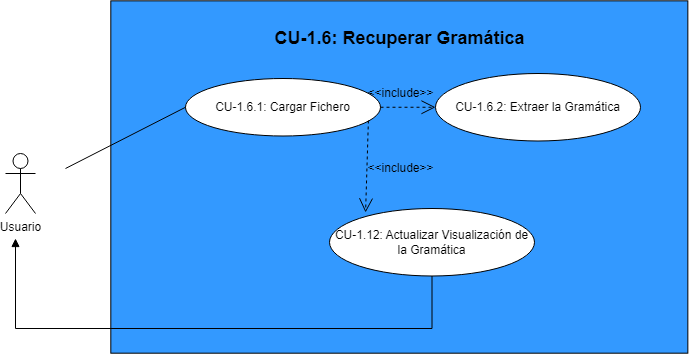
\includegraphics[scale=0.55]{figuras/Cap7/CU16.png}
 	\caption{CU-1.6: Recuperar gramática}
 	\label{fig:CU16}
       \end{center}
   \end{figure}

 \begin{longtable}[H]{|>{\columncolor[rgb]{0.63,0.79,0.95}}m{6cm} | m{8.5cm} |}
 \caption{Caso de uso: CU-1.6 Recuperar gramática} \\
 \endfirsthead
 \multicolumn{2}{c}
 {{ \tablename\ \thetable{} -- continúa de la página anterior}} \\
 \endhead
 \hline \multicolumn{2}{|r|}{{continúa en la página siguiente}} \\ \hline
 \endfoot
 \hline
 \endlastfoot
  \hline
  \textbf{Nombre} & \textbf{CU-1.6 Recuperar gramática}.\newline \textbf{Nivel}: 2  \\ \hline
  \textbf{Descripción} & Permite al usuario recuperar una gramática de un fichero.\\ \hline
  \textbf{Actores} & Usuario \\ \hline
  \textbf{Casos de uso} & 
     \begin{enumerate}
     \item \textbf{CU-1.6.1 Cargar fichero}: \textit{carga} un fichero que contiene una gramática.
     \item \textbf{CU-1.6.2 Extraer la gramática}:  \textit{extrae} la gramática contenida en el fichero recuperado.
     \item \textbf{CU-1.12. Actualizar visualización de la gramática}: \textit{actualiza} la visualización de la gramática en la interfaz del simulador.
     \end{enumerate} \\ \hline
  \textbf{Flujo de eventos principal} & 
     \begin{enumerate}
     \item El usuario \textit{selecciona} el fichero que contiene la gramática que desea cargar.
     \item Se \textit{extrae} la gramática del fichero.
     \item Se \textit{carga} la gramática en el editor (creando toda la estructura de la gramática y actualizando la vista de la gramática pertinente).
     \end{enumerate}\\ \hline
  \textbf{Flujo de eventos alternativo} & Si se produce algún fallo durante el paso 1, se procede como sigue: 
     \begin{enumerate}
     \item Se \textit{informa} al usuario de que no ha podido seleccionar ningún fichero. 
     \item Se \textit{termina} la acción de recuperar gramática.
     \end{enumerate}  \\ \hline
  \textbf{Flujo de eventos alternativo} & Si se produce algún fallo durante el paso 2, se procede como sigue:
     \begin{enumerate}
     \item Se \textit{informa} al usuario de que la gramática no pudo ser extraída o cargada en  el simulador, debido a posibles problemas en la estructura del archivo.
     \item Se \textit{termina} la acción de recuperar gramática.
     \end{enumerate} \\ \hline          
   \textbf{Flujo de eventos alternativo} & Si se produce algún fallo durante el paso 3, se procede como sigue:
         \begin{enumerate}
         \item Se \textit{informa} al usuario de que la gramática ha podido ser extraída pero no se puede cargar en el editor.
         \item Se \textit{termina} la acción de recuperar gramática.
         \end{enumerate}
   \label{tabla77}
 \end{longtable}

 Los casos de uso \textit{CU-1.6.1 Cargar fichero} y \textit{CU-1.6.2 Extraer gramática} no se refinarán más, puesto que son casos de uso bastante sencillos y que pueden ser fácilmente traducidos a una implementación posterior sin necesidad de ser refinados.

 \subsubsection{CU-1.7. Guardar gramática}

 Este caso de uso representa el almacenamiento de una gramática. En la figura \ref{fig:CU17} se muestra la representación gráfica del caso de uso y en la tabla \ref{tabla78} se muestra su representación tabular. 

   \begin{figure}[H]
       \begin{center} 
 	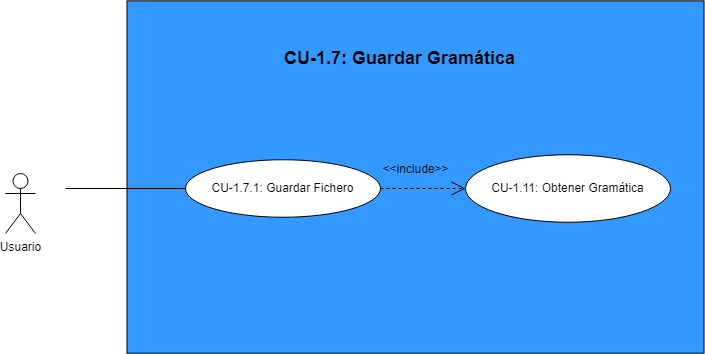
\includegraphics[scale=0.55]{figuras/Cap7/CU17.png}
 	\caption{CU-1.7: Guardar gramática}
 	\label{fig:CU17}
       \end{center}
   \end{figure}
  
   \newpage

 \begin{longtable}[H]{|>{\columncolor[rgb]{0.63,0.79,0.95}}m{6cm} | m{8.5cm} |} 
 \caption{Caso de uso: CU-1.7 Guardar gramática} \\
 \endfirsthead
 \multicolumn{2}{c}
 {{ \tablename\ \thetable{} -- continúa de la página anterior}} \\
 \endhead
 \hline \multicolumn{2}{|r|}{{continúa en la página siguiente}} \\ \hline
 \endfoot
 \hline
 \endlastfoot

  \hline
  \textbf{Nombre} & \textbf{CU-1.7 Guardar gramática}.\newline \textbf{Nivel}: 2  \\ \hline
   \textbf{Descripción} & Permite al usuario guardar una gramática de un fichero.\\ \hline                    
  \textbf{Actores} & Usuario \\ \hline
  \textbf{Casos de uso} & 
     \begin{enumerate}
     \item \textbf{CU-1.7.1 Guardar fichero}: \textit{guarda} en un fichero la gramática creada.
     \item \textbf{CU-1.11. Obtener gramática}: \textit{obtiene} el vocabulario de símbolos ($V_{N}, V_{T}$) así como las producciones de la gramática.
     \end{enumerate} \\ \hline
  \textbf{Flujo de eventos principal} & 
     \begin{enumerate}
     \item El usuario \textit{selecciona} el fichero en el que desea guardar la gramática.
     \item Se \textit{guarda} la gramática en un fichero (con el formato especificado en el capítulo anterior).
     \end{enumerate}\\ \hline
  \textbf{Flujo de eventos alternativo} & Si se produce algún fallo durante el paso 1, se procede como sigue:
     \begin{enumerate}
     \item Se \textit{informa} al usuario de que no ha podido seleccionar crear el fichero.
     \item Se \textit{termina} la acción de guardar gramática.
     \end{enumerate}  \\ \hline
  \textbf{Flujo de eventos alternativo} & Si se produce algún fallo durante el paso 2, se procede como sigue:
     \begin{enumerate}
     \item Se \textit{informa} al usuario de que la gramática no pudo ser guardada.
     \item Se \textit{termina} la acción de guardar gramática.
     \end{enumerate} 
   \label{tabla78}
 \end{longtable}

 El caso de uso \textit{CU-1.7.1 Guardar fichero} no se refinará más, puesto que se trata de un proceso simple que puede ser fácilmente traducido a una implementación posterior sin necesidad de ser refinado más.

 \subsubsection{CU-1.8. Validar gramática}

 Este caso de uso representa la validación de una gramática. En la figura \ref{fig:CU18} se muestra la representación gráfica del caso de uso y en la tabla \ref{tabla79} se muestra su representación tabular.

 \begin{figure}[H]
       \begin{center} 
 	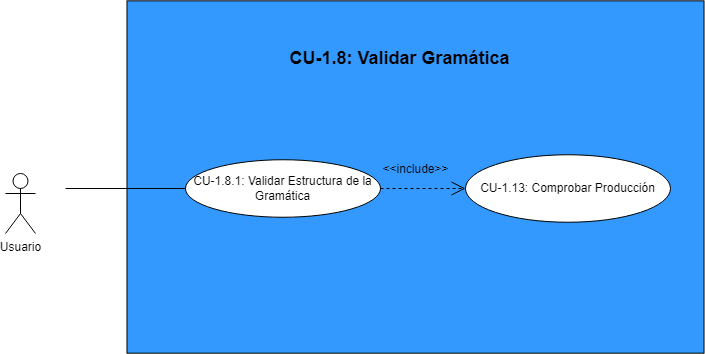
\includegraphics[scale=0.55]{figuras/Cap7/CU18.png}
 	\caption{CU-1.8: Validar gramática}
 	\label{fig:CU18}
       \end{center}
   \end{figure}
  
   \newpage

 \begin{longtable}[H]{|>{\columncolor[rgb]{0.63,0.79,0.95}}m{6cm} | m{8.5cm} |}
 \caption{Caso de uso: CU-1.8 Validar gramática} \\
 \endfirsthead
 \multicolumn{2}{c}
 {{ \tablename\ \thetable{} -- continúa de la página anterior}} \\
 \endhead
 \hline \multicolumn{2}{|r|}{{continúa en la página siguiente}} \\ \hline
 \endfoot
 \hline
 \endlastfoot
  \hline
  \textbf{Nombre} & \textbf{CU-1.8 Validar gramática}.\newline \textbf{Nivel}: 2  \\ \hline
  \textbf{Descripción} & Permite al usuario validar una gramática de contexto libre.\\ \hline
  \textbf{Actores} & Usuario \\ \hline
  \textbf{Casos de uso} & 
     \begin{enumerate}
     \item \textbf{CU-1.8.1 Validar estructura de la gramática}: \textit{valida} la estructura  de la gramática, formada por el conjunto de producciones, símbolos (\textit{terminales} y \textit{no terminales}) y símbolo inicial.
     \item \textbf{CU-1.12 Comprobar producción}: \textit{comprueba} si una producción es correcta.
     \end{enumerate} \\ \hline                             
  \textbf{Flujo de eventos principal} & 
     \begin{enumerate}
     \item Se \textit{obtiene} todo el vocabulario de la gramática a ser validada. 
     \item Se \textit{comprueban} todas las producciones que componen la gramática.
     \item Se \textit{informa} al usuario acerca del resultado del la validación.
     \end{enumerate}\\ \hline                 
  \textbf{Flujo de eventos alternativo} & Si se produce algún fallo durante el paso 1, se procede como sigue:
     \begin{enumerate}
     \item Se \textit{informa} al usuario de que no ha podido obtener el vocabulario de  la gramática.
     \item Se \textit{termina} la acción de validar gramática.
     \end{enumerate}  \\ \hline          
  \textbf{Flujo de eventos alternativo} & Si se produce algún fallo durante el paso 2, se procede como sigue:
     \begin{enumerate}
     \item Se \textit{informa} al usuario de que no se han podido comprobar las producciones de  la gramática.
     \item Se \textit{termina} la acción de validar gramática.
     \end{enumerate} \\ \hline         
  \textbf{Flujo de eventos excepcional} & Si durante la ejecución del paso 2, alguna producción comprobada posee e\-rro\-res (esto excluye cualquier error de funcionamiento, des\-cri\-to en el flujo alternativo anterior), se procede como sigue:
     \begin{enumerate}
     \item El \textit{resultado} de la validación será insatisfactorio.
     \end{enumerate}
   \label{tabla79}
 \end{longtable}

 El caso de uso \textit{CU-1.8.1 Validar estructura de la gramática} no se refinará más, puesto que es un proceso simple que puede ser fácilmente traducido a una implementación posterior sin necesidad de ser refinado más.

 \subsubsection{CU-1.9. Generar informe de gramática}
 
 Este caso de uso representa la generación de un informe de una gramática. En la figura \ref{fig:CU19} se muestra la representación gráfica del caso de uso y en la  tabla \ref{tabla710} se muestra su representación tabular.

  \begin{figure}[H]
       \begin{center} 
 	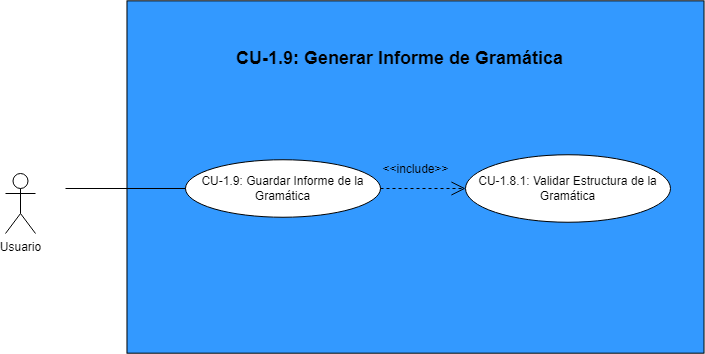
\includegraphics[scale=0.55]{figuras/Cap7/CU19.png}
 	\caption{CU-1.9: Generar informe de gramática}
 	\label{fig:CU19}
       \end{center}
   \end{figure}

 \begin{longtable}[H]{|>{\columncolor[rgb]{0.63,0.79,0.95}}m{6cm} | m{8.5cm} |}
 \caption{Caso de uso: CU-1.9 Generar informe de gramática} \\
 \endfirsthead
 \multicolumn{2}{c}
 {{ \tablename\ \thetable{} -- continúa de la página anterior}} \\
 \endhead
 \hline \multicolumn{2}{|r|}{{continúa en la página siguiente}} \\ \hline
 \endfoot
 \hline
 \endlastfoot
  \hline
  \textbf{Nombre} & \textbf{CU-1.9 Generar informe de gramática}. \newline \textbf{Nivel}: 2  \\ \hline
  \textbf{Descripción} & Permite al usuario generar un informe de una gramática.\\ \hline                       
  \textbf{Actores} & Usuario \\ \hline
  \textbf{Casos de uso} & 
     \begin{enumerate}
     \item \textbf{CU-1.9.1 Guardar informe de la gramática}: \textit{guarda} un fichero que  contiene el informe de la gramática.
     \item \textbf{CU-1.8.1 Validar estructura de la gramática}: \textit{valida} la estructura  de la gramática, formada por el conjunto de producciones y símbolos (\textit{terminales} y \textit{no terminales}).
     \end{enumerate} \\ \hline
 
  \textbf{Flujo de eventos principal} & 
         \begin{enumerate}
         \item Se re\-a\-li\-za una \textit{validación} de la estructura de la gramática, para así  comprobar si la gramática es co\-rrec\-ta.
         \item Se \textit{genera} un informe de la gramática, según lo especificado en \textit{RI- INF-1}.
         \end{enumerate}\\ \hline             
  \textbf{Flujo de eventos alternativo} & Si se produce algún fallo durante el paso 1, se procede como sigue:
     \begin{enumerate}
     \item Se \textit{informa} al usuario que no ha podido generar el informe de la gramática.
     \item Se \textit{termina} la acción de generar informe de gramática.
     \end{enumerate}   \\ \hline              
  \textbf{Flujo de eventos alternativo} & Si se produce algún fallo durante el paso 2, se procede como sigue:
     \begin{enumerate}
     \item Se \textit{informa} al usuario de que el informe no ha podido ser guardado.
     \item Se \textit{termina} la acción de generar informe de gramática.
     \end{enumerate}  \\ \hline
  \textbf{Flujo de eventos excepcional} & Si durante la ejecución del paso 1, se detecta que la gramática no es válida, puesto que posee errores (esto excluye cualquier error de funcionamiento, descrito en el flujo alternativo anterior), se procede como sigue:
     \begin{enumerate}
     \item Se \textit{aborta} la generación del informe.
     \item Se \textit{informa} al usuario de que la gramática contiene errores.
     \end{enumerate}
   \label{tabla710}
 \end{longtable}

 El caso de uso \textit{CU-1.9.1 Guardar informe de la gramática} no se refinará más, puesto que es un \textbf{proceso simple} que puede ser fácilmente traducido a una implementación posterior sin necesidad de ser refinado.

 \subsubsection{CU-1.10. Transferir al simulador}

 Este caso de uso representa la transferencia de una gramática al simulador. En la figura \ref{fig:CU110} se muestra la representación gráfica del caso de uso y en la tabla \ref{tabla711} se muestra su representación tabular.

 \begin{figure}[H]
       \begin{center} 
 	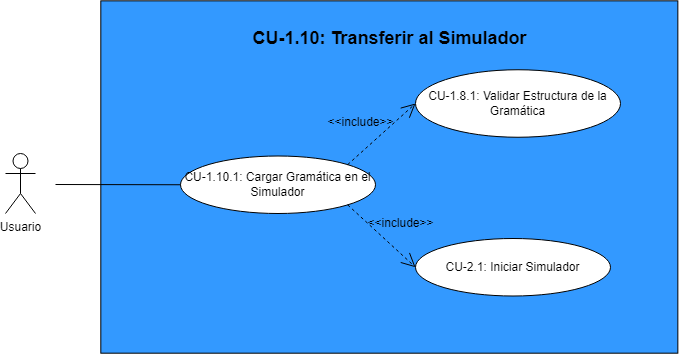
\includegraphics[scale=0.55]{figuras/Cap7/CU110.png}
 	\caption{CU-1.10: Transferir al simulador}
 	\label{fig:CU110}
       \end{center}
   \end{figure}

 \begin{longtable}[H]{|>{\columncolor[rgb]{0.63,0.79,0.95}}m{6cm} | m{8.5cm} |}
 \caption{Caso de uso: CU-1.10 Transferir al simulador} \\
 \endfirsthead
 \multicolumn{2}{c}
 {{ \tablename\ \thetable{} -- continúa de la página anterior}} \\
 \endhead
 \hline \multicolumn{2}{|r|}{{continúa en la página siguiente}} \\ \hline
 \endfoot
 \hline
 \endlastfoot
  \hline
  \textbf{Nombre} & \textbf{CU-1.10 Transferir al simulador}.\newline \textbf{Nivel}: 2  \\ \hline
  \textbf{Descripción} & Permite al usuario transferir una gramática al simulador para simular un método de  análisis sintáctico.\\ \hline
  \textbf{Actores} & Usuario \\ \hline
  \textbf{Casos de uso} & 
     \begin{enumerate}
     \item \textbf{CU-1.10.1 Cargar gramática en el simulador}: \textit{carga} la gramática en  el si\-mu\-la\-dor.
     \item \textbf{CU-1.8.1 Validar estructura de la gramática}: \textit{valida} la estructura  de la gramática, formada por el conjunto de producciones y símbolos (\textit{terminales} y \textit{no terminales}).
     \item \textbf{CU-2.1. Iniciar el simulador}: \textit{i\-ni\-cia\-li\-za} el simulador y  transfiere la gramática, o simplemente carga la gramática en el simulador (en el caso de que este ya se encuentre ini\-cia\-li\-zado previamente).
     \end{enumerate} \\ \hline                             
  \textbf{Flujo de eventos principal} & 
     \begin{enumerate}
     \item Se \textit{re\-a\-li\-za} una validación de la estructura de la gramática, para así  comprobar si la gramática es co\-rre\-cta.
     \item Se \textit{transfiere} la gramática al si\-mu\-la\-dor y se ini\-cia\-li\-za este (en caso de que no se haya iniciado anteriormente al transferir otra gramática)
     \end{enumerate}\\ \hline
  \textbf{Flujo de eventos alternativo} & Si se produce algún fallo durante el paso 1, se procede como sigue:
     \begin{enumerate}
     \item Se \textit{informa} al usuario de que no ha podido validar la gramática.
     \item Se \textit{termina} la acción de transferir al si\-mu\-la\-dor.
     \end{enumerate}  \\ \hline              
  \textbf{Flujo de eventos alternativo} & Si se produce algún fallo durante el paso 2, se procede como sigue:
     \begin{enumerate}
     \item Se \textit{informa} al usuario de que no se ha podido transferir la gramática.
     \item Se \textit{termina} la acción de transferir al si\-mu\-la\-dor.
     \end{enumerate}  \\ \hline             
  \textbf{Flujo de eventos excepcional} & Si durante la ejecución del paso 1, se detecta que la gramática no es válida, puesto que posee errores (esto excluye cualquier error de funcionamiento, des\-cri\-to en el flujo alternativo anterior), se procede como sigue: 
     \begin{enumerate}
     \item Se \textit{aborta} la transferencia de la gramática.
     \item Se \textit{informa} al usuario de que la gramática contiene errores (no es una gramática válida).
     \end{enumerate}
   \label{tabla711}
 \end{longtable}

 El caso de uso \textit{CU-1.10.1 Cargar gramática en el simulador} no se refinará más, puesto que se trata de un proceso simple, que puede ser fácilmente traducido a una implementación posterior sin necesidad de ser refinado.

 \subsubsection{CU-1.11. Obtener gramática}

 Este caso de uso se encarga de obtener el vocabulario de la gramática $ (V_{N}, V_{T}) $, así como todo el conjunto de producciones y el símbolo inicial.

 Se trata de un proceso bastante sencillo, pero que es utilizado en los demás casos de uso cada vez que se desea obtener la estructura de una gramática. Este caso de uso será directamente traducido a una implementación sin ser preciso re\-a\-li\-zar un refinamiento más exhaustivo.

 \subsubsection{CU-1.12. Actualizar visualización}

 Este caso de uso representa la actualización de la visualización de una gramática. Cabe destacar que este caso de uso no es invocado directamente por el usuario, sino que el propio Sistema actualiza la vista de la gramática automáticamente, a medida que esta sufre alguna modificación (a partir de aquellos casos de uso que incluyen el comportamiento de este caso de uso). En la figura \ref{fig:CU112} se muestra la representación gráfica del caso de uso y en la  tabla \ref{tabla712} se muestra su representación tabular.

  \begin{figure}[H]
       \begin{center} 
 	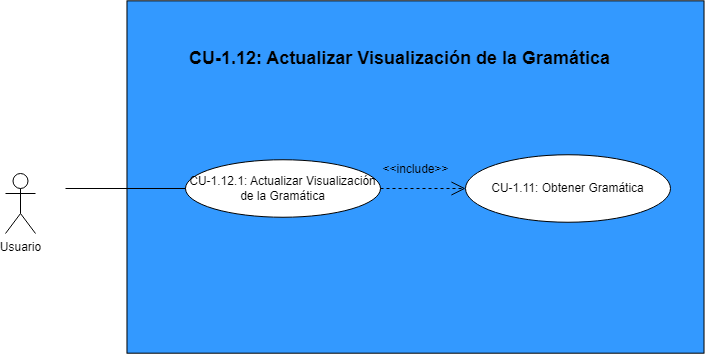
\includegraphics[scale=0.55]{figuras/Cap7/CU112.png}
 	\caption{CU-1.12: Actualizar visualización de la gramática}
 	\label{fig:CU112}
       \end{center}
   \end{figure}

 \begin{longtable}[H]{|>{\columncolor[rgb]{0.63,0.79,0.95}}m{6cm} | m{8.5cm} |}
 \caption{Caso de uso: CU-1.12 Actualizar visualización de la gramática} \\
 \endfirsthead
 \multicolumn{2}{c}
 {{ \tablename\ \thetable{} -- continúa de la página anterior}} \\
 \endhead
 \hline \multicolumn{2}{|r|}{{continúa en la página siguiente}} \\ \hline
 \endfoot
 \hline
 \endlastfoot
  \hline
  \textbf{Nombre} & \textbf{CU-1.12 Actualizar visualización de la gramática}.\newline \textbf{Nivel}: 2  \\ \hline
  \textbf{Descripción} & Permite al usuario visualizar la gramática a medida que la va construyendo.\\ \hline                       
  \textbf{Actores} & Usuario \\ \hline
  \textbf{Casos de uso} & 
     \begin{enumerate}
     \item \textbf{CU-1.12.1 Actualizar vi\-sua\-li\-za\-ción de la gramática}: \textit{ac\-tua\-li\-za} la vi\-sua\-li\-za\-ción de la gramática en el editor, a medida que esta sufre alguna modificación en su estructura (producciones y símbolos).
     \item \textbf{CU-1.11. gramática}: \textit{obtiene} el vocabulario de símbolos ($V_{N}, V_{T}$) así como las producciones de la gramática.
     \end{enumerate} \\ \hline
  \textbf{Flujo de eventos principal} & 
     \begin{enumerate}
     \item Se \textit{obtiene} el vocabulario de la gramática.               \item Se \textit{actualiza} la vista de la gramática en el editor de gramáticas.
     \end{enumerate}\\ \hline                     
  \textbf{Flujo de eventos alternativo} & Si se produce algún fallo durante el paso 1, se procede como sigue:
     \begin{enumerate}
     \item Se \textit{informa} al usuario de que no ha podido obtener el vocabulario de la  	gramática y que existen errores que impiden vi\-sua\-li\-zar\-la.
     \item Se \textit{aborta} la actualización de la vista de la gramática.
     \end{enumerate}  \\ \hline              
  \textbf{Flujo de eventos alternativo} & Si se produce algún fallo durante el paso 2, se procede como sigue:
     \begin{enumerate}
     \item Se \textit{informa} al usuario de que no ha podido actualizar la vista de la gramática.
     \item Se \textit{aborta} la actualización de la vista de la gramática.
     \end{enumerate}  
   \label{tabla712}
 \end{longtable}

 El casos de uso \textit{CU-1.12.1 Actualizar visualización de la gramática} no se refinará más, puesto que se trata de un proceso simple, que puede ser fácilmente traducido a una  implementación posterior sin necesidad de ser refinado.

 \subsubsection{CU-1.13. Comprobar producción}

 Este caso de uso se encargará de comprobar si la estructura de una regla gramatical o producción es correcta. 

 No es necesario refinar de forma profunda este caso de uso ya que es bastante simple y no depende de ningún caso de uso de nivel inferior, por lo que se puede traducir fácilmente sin un mayor refinamiento.

 \subsection{CU-2. Simular análisis sintáctico descendente predictivo}

Este caso de uso representa la simulación del análisis sintáctico descendente predictivo con una gramática de contexto libre. En la figura \ref{fig:CU2} se muestra la representación gráfica de este caso de uso, que está formada por los siguientes sub-casos de uso:

 \begin{itemize}
  \item \textbf{CU-2.1. Simular Análisis Descendente Predictivo}.
  \item \textbf{CU-2.2. Buscar Gramática}.
  \item \textbf{CU-2.3. Completar Tabla con Funciones de Error}.
  \item \textbf{CU-2.4. Analizar Cadena}.
  \item \textbf{CU-2.5. Seleccionar Velocidad Simulación}.
  \item \textbf{CU-2.6. Construir Árbol Sintáctico}.
  \item \textbf{CU-2.7. Mostrar la derivación}.
  \item \textbf{CU-2.8. Generar Informe Simulación}.
 \end{itemize}

 \begin{figure}[H]
       \begin{center} 
 	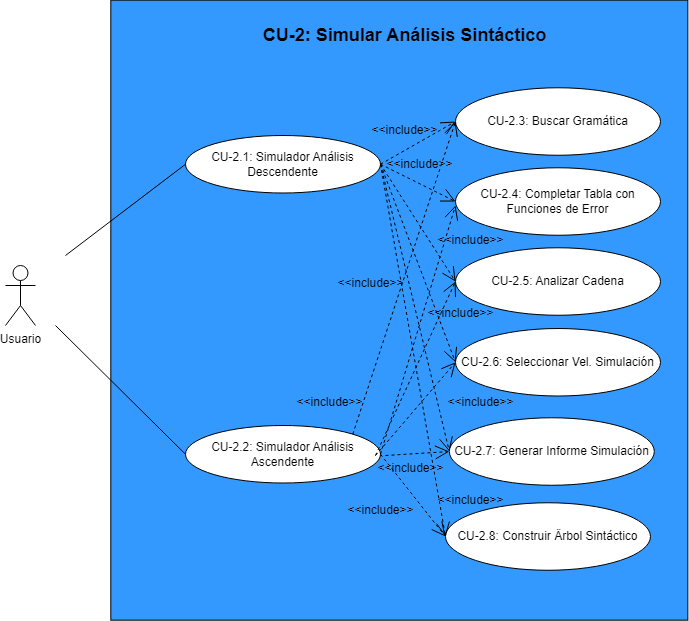
\includegraphics[scale=0.55]{figuras/Cap7/CU2.png}
 	\caption{CU-2 Simular análisis sintáctico predictivo}
 	\label{fig:CU2}
       \end{center}
   \end{figure}
  
 La especificación del caso de uso se muestra en la tabla \ref{tabla715}.

 \begin{longtable}[H]{|>{\columncolor[rgb]{0.63,0.79,0.95}}m{6cm} | m{8.5cm} |}
 \caption{Caso de uso: CU-2 Simular análisis sintáctico} \\
 \endfirsthead
 \multicolumn{2}{c}
 {{ \tablename\ \thetable{} -- continúa de la página anterior}} \\
 \endhead
 \hline \multicolumn{2}{|r|}{{Continúa en la página siguiente}} \\ \hline
 \endfoot
 \hline
 \endlastfoot
  \hline
  \textbf{Nombre} & \textbf{CU-2. Simular análisis sintáctico}. \newline \textbf{Nivel}: 1  \\ \hline
   \textbf{Descripción} & Permite al usuario realizar la simulación de un analizador sintáctico usando  una gramática.\\ \hline
  \textbf{Actores} & Usuario \\ \hline 
  \textbf{Casos de uso} & 
     \begin{enumerate}
     \item \textbf{CU-2.1. Simular Análisis Descendente Predictivo}: lleva a cabo el análisis sintáctico descendente predictivo de una gramática de contexto libre.
     \item \textbf{CU-2.2. Buscar gramática}: realiza la búsqueda en el sistema de una gramática de contexto libre guardada con anterioridad.
     \end{enumerate} \\ \hline
                                 
  \textbf{Flujo de eventos principal} & 
     \begin{enumerate}
     \item Se \textit{selecciona} la gramática que se desea simular.
     \item Se \textit{realiza} el análisis sintáctico descendente predictivo.
     \end{enumerate}\\ \hline
  \textbf{Flujo de eventos alternativo} & Si se produce un fallo durante el paso 1, se procede como sigue:
     \begin{enumerate}
     \item Se \textit{informa} al usuario que se ha podido cargar la gramática seleccionada.
     \item Se \textit{aborta} la selección de la gramática y no se podrá llevar a cabo la  simulación de dicha gramática.
     \item Se redirecciona a la pantalla de simulación.
     \end{enumerate}   
   \label{tabla715}
 \end{longtable}

 A continuación, se refinará cada uno de los casos de uso que componen el caso de uso CU-2.

 \subsubsection{CU-2.1. Simular Análisis Descendente Predictivo}

 Este caso de uso representa la simulación del análisis sintáctico descendente predictivo de una gramática de contexto libre. En la figura \ref{fig:CU21} se muestra la representación gráfica del caso de uso y en la  tabla \ref{tabla716} se muestra su representación tabular. Los sub-casos de uso que lo conforman son:

 \begin{itemize}
  \item \textbf{CU-2.1.1 Gestionar Tabla Predictiva}.
  \item \textbf{CU-2.1.2 Gestionar Conjunto Primero y Siguiente}.
 \end{itemize}

Este caso de uso CU-2.1 también interactúa con los siguientes casos de uso:
 \begin{itemize}
  \item \textbf{CU-2.2. Buscar Gramática}.
  \item \textbf{CU-2.3. Completar Tabla con Funciones de Error}.
  \item \textbf{CU-2.4. Analizar Cadena}.
  \item \textbf{CU-2.5. Seleccionar Velocidad Simulación}.
  \item \textbf{CU-2.6. Generar Informe Simulación}.
  \item \textbf{CU-2.7. Construir Árbol Sintáctico}.
 \end{itemize}


  \begin{figure}[H]
       \begin{center} 
 	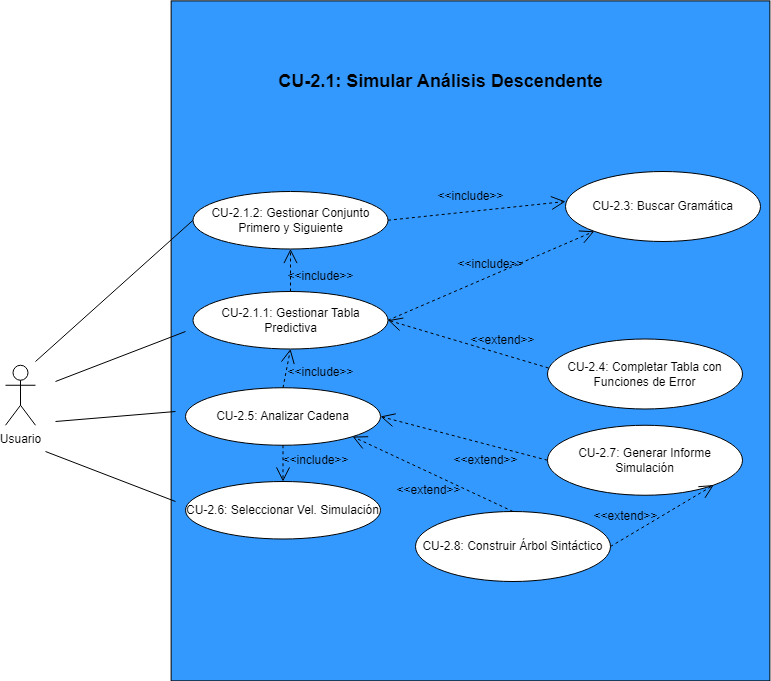
\includegraphics[scale=0.55]{figuras/Cap7/CU21.png}
 	\caption{CU-2.1 Simular Análisis descendente}
 	\label{fig:CU21}
       \end{center}
   \end{figure}
  
 \begin{longtable}[H]{|>{\columncolor[rgb]{0.63,0.79,0.95}}m{6cm} | m{8.5cm} |}
 \caption{Caso de uso: CU-2.1 Simular Análisis descendente predictivo} \\
 \endfirsthead
 \multicolumn{2}{c}
 {{ \tablename\ \thetable{} -- continúa de la página anterior}} \\
 \endhead
 \hline \multicolumn{2}{|r|}{{Continúa en la página siguiente}} \\ \hline
 \endfoot
 \hline
 \endlastfoot
  \hline
  \textbf{Nombre} & \textbf{CU-2.1. Simular Análisis descendente}. \newline \textbf{Nivel}: 2  \\ \hline
  \textbf{Descripción} & Permite al usuario realizar la simulación del análisis sintáctico descendente de una gramática de contexto libre.\\ \hline                 
  \textbf{Actores} & Usuario \\ \hline
  \textbf{Casos de uso} & 
     \begin{enumerate}
     \item \textbf{CU-2.1.1. Gestionar tabla predictiva}: \textit{gestionar} la tabla predictiva  necesaria para llevar a cabo la simulación.
     \item \textbf{CU-2.3. Buscar gramática}: realiza la búsqueda en el sistema de una gramática de contexto libre guardada con anterioridad.
     \item \textbf{CU-2.4. Completar tabla con funciones de error}: si el usuario lo desea, puede \textit{completar} la tabla predictiva con funciones para el tratamiento de los errores  que se 	puedan producir.
     \item \textbf{CU-2.1.2. Gestionar conjunto primero y siguiente}: \textit{gestionar} el  conjunto primero y siguiente de una gramática de contexto libre, necesarios para crear la tabla predictiva.			  
     \item \textbf{CU-2.5. Analizar cadena}: \textit{realiza} el análisis sintáctico descendente predictivo de una cadena.
     \item \textbf{CU-2.6. Seleccionar velocidad de simulación}: \textit{selecciona} la velocidad a la que se llevará a cabo la simulación: paso a paso o continua.
     \item \textbf{CU-2.7. Generar informe de la simulación}: una vez terminado el proceso de simulación, el usuario puede obtener un informe con todos los detalles.
     \item \textbf{CU-2.8. Construir Árbol Sintáctico}: se construirá el árbol sintáctico de la derivación correspondiente.
     \end{enumerate} \\ \hline
                                 
  \textbf{Flujo de eventos principal} & 
     \begin{enumerate}
     \item Se \textit{selecciona} la gramática que se desea simular.
     \item Se \textit{construye} el conjunto primero y siguiente.\item Se \textit{crea} la tabla predictiva con los datos de los pasos anteriores.
     \item Si se desea, se puede \textit{completar} la tabla predictiva con funciones de tratamiento de errores.
     \item Una vez que se tiene todo lo anterior, se procede a analizar una cadena con el simulador.
     \item Se \textit{elige} la velocidad de simulación: paso a paso o continua.
     \item Se \textit{escoge} si se desea construir de forma paralela a la derivación el árbol sintáctico.
     \item Se \textit{genera} el informe de la simulación que se ha llevado a cabo en los pasos anteriores.
     \end{enumerate}\\ \hline
                     
  \textbf{Flujo de eventos alternativo} & Si se produce un fallo durante el paso 1, se procede como sigue:
     \begin{enumerate}
     \item Se \textit{informa} al usuario que no se ha podido cargar la gramática seleccionada.
     \item Se \textit{aborta} la selección de la gramática y no se podrá llevar a cabo la  simulación.
     \item Se redirecciona a la pantalla de simulación.			\end{enumerate}    \\ \hline
  \textbf{Flujo de eventos alternativo} & Si se produce un fallo durante el paso 3, se procede como sigue:
     \begin{enumerate}
     \item Se \textit{informa} al usuario que se ha podido crear la tabla predictiva.
     \item Se \textit{aborta} la creación de la tabla predictiva y no se podrá llevar a cabo la simulación hasta que todos los datos sean correctos.
     \item Se redirecciona a la pantalla de simulación.
     \end{enumerate}   \\ \hline
  \textbf{Flujo de eventos alternativo} & Si se produce un fallo durante el paso 5, se procede como sigue:
     \begin{enumerate}
     \item Se \textit{informa} al usuario que no se ha podido analizar la cadena introducida.
     \item Se \textit{aborta} el análisis y no se podrá llevar a cabo hasta que todos los datos sean correctos.
     \item Se redirecciona a la pantalla de simulación.			\end{enumerate}   \\ \hline
 \textbf{Flujo de eventos alternativo} & Si se produce un fallo durante el paso 7, se procede como sigue:
     \begin{enumerate}
     \item Se \textit{informa} al usuario que no se ha podido generar el informe de la simulación.
     \item Se \textit{aborta} la generación del informe y no se podrá obtener el informe.
     \item Se redirecciona a la pantalla de simulación.			\end{enumerate}
   \label{tabla716}
 \end{longtable}

 El caso de uso \textit{CU-2.1.1} no se refinará más, puesto que se trata de un proceso simple, que puede ser fácilmente traducido a una implementación posterior sin necesidad de ser refinado.


\subsubsection{CU-2.1.2. Gestionar conjunto Primero y Siguiente}

Este caso de uso es un proceso simple que consiste en crear los conjuntos primero y siguiente de la gramática, necesarios para crear las tablas de análisis en el análisis sintáctico descendente predicitivo. Por tanto, este proceso no será refinado de forma más exhaustiva.

\subsubsection{CU-2.2. Buscar gramática}

Este caso de uso es un proceso simple que consiste en seleccionar una gramática de entre las que se encuentran cargadas en el simulador. Por tanto, este proceso no será refinado de forma más exhaustiva.


\subsubsection{CU-2.3. Completar tabla con funciones de error}

Este caso de uso es un proceso simple en el cual, una vez construida la tabla del análisis sintáctico, se completa con la funciones de error. Por tanto, este proceso no será refinado de forma más exhaustiva.

 \subsubsection{CU-2.4. Analizar cadena}

 Este caso de uso es un proceso simple en el que se lleva a cabo el análisis sintáctico descendente de una cadena. Por tanto, este proceso no será refinado de forma más exhaustiva.

 \subsubsection{CU-2.5. Selecciona velocidad de simulación}

 Este caso de uso es un proceso simple que consiste en seleccionar entre los dos tipos de velocidad de simulación: paso a paso o continuo. Por tanto, este proceso no será refinado de forma más exhaustiva.

 \subsubsection{CU-2.6. Generar informe de simulación}

 Este caso de uso es un proceso simple que consiste en generar un informe con todos los datos del análisis sintáctico creados durante la simulación, el cual podrá ver y descargar el usuario. Por tanto, este proceso no será refinado de forma más exhaustiva.

 \subsubsection{CU-2.7. Construir Árbol Sintáctico Descendente}

 Este caso de uso es un proceso simple que consiste en generar la construcción del árbol sintáctico descendente correspondiente a la derivación que se está realizando en dicho momento. Esta generación del árbol puede ser tanto instantánea como paso a paso y se hará de forma paralela a la propia derivación.


 \subsection{CU-3. Consultar Tutorial}

 Este caso de uso representa la consulta del tutorial de la aplicación. En la figura \ref{fig:CU3} se muestra la representación gráfica de este caso de uso, que está formada por los siguientes sub-casos de uso:

 \begin{itemize}
  \item \textbf{CU-3.1. Consultar una lección}.
  \item \textbf{CU-3.2. Obtener recurso del tutorial}.
  \item \textbf{CU-3.3. Navegar por el recurso seleccionado}.

 \end{itemize}

 En este caso de uso se muestran flechas que se dirige desde un caso de uso al usuario. Esto representa el hecho de que el usuario visualiza el tutorial por pantalla.

  \begin{figure}[H]
       \begin{center} 
 	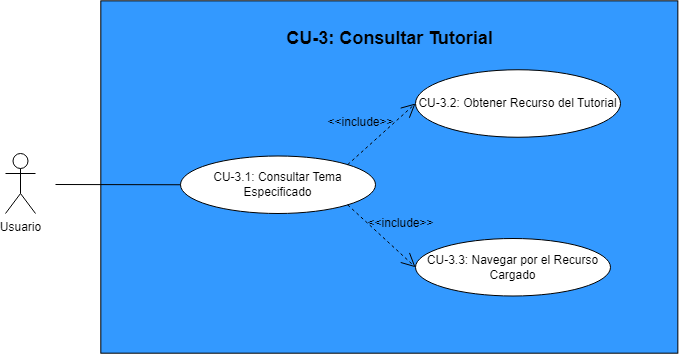
\includegraphics[scale=0.55]{figuras/Cap7/CU3.png}
 	\caption{CU-3: Consultar Tutorial}
 	\label{fig:CU3}
       \end{center}
   \end{figure}

 La especificación del caso de uso se muestra en la tabla \ref{tabla713}.


 \begin{longtable}[H]{|>{\columncolor[rgb]{0.63,0.79,0.95}}m{6cm} | m{8.5cm} |}
 \caption{Caso de uso: CU-3. Consultar Tutorial} \\

 \endfirsthead

 \multicolumn{2}{c}
 {{ \tablename\ \thetable{} -- continúa de la página anterior}} \\
 \endhead
 \hline \multicolumn{2}{|r|}{{Continúa en la página siguiente}} \\ \hline
 \endfoot
 \hline
 \endlastfoot
  \hline
  \textbf{Nombre} & \textbf{CU-3. Consultar Tutorial}.\newline \textbf{Nivel}: 1  \\ \hline
  \textbf{Descripción} & Permite al usuario consultar el tutorial de la aplicación.\\ \hline
  \textbf{Actores} & Usuario \\ \hline
  \textbf{Casos de uso} & 
     \begin{enumerate}
     \item \textbf{CU-3.1. Consultar una lección}: permite \textit{consultar} una lección del tutorial.
     \item \textbf{CU-3.2. Obtener recurso del tutorial}: permite \textit{obtener} una lección del tutorial. 
     \item \textbf{CU-3.3. Navegar por el recurso seleccionado}: permite \textit{navegar} por una lección del tutorial.
     \end{enumerate} \\ \hline
                                 
  \textbf{Flujo de eventos principal} & 
     \begin{enumerate}
     \item Se \textit{obtiene} un recurso del tutorial (especificado por el usuario).
     \item El usuario \textit{navega} por el recurso.
     \item El usuario \textit{accede} a otro recurso a través del enlace (para lo que se vuelve al paso 1), o sigue navegando por el mismo.
     \end{enumerate}\\ \hline
                     
  \textbf{Flujo de eventos alternativo} & Si se produce algún error al \textit{cargar} o \textit{navegar} por un recurso del tutorial, se informa al usuario y se restablece el recurso previo (cerrando el tutorial en caso de que se produzca un fallo).
   \label{tabla713}
 \end{longtable}

Nótese que lo que aquí se llama recurso del tutorial, es realmente una \textit{lección} del tutorial. El hecho de de\-no\-mi\-nar\-lo recurso implica que el fichero en cuestión (un recurso del simulador) es buscado y cargado, y, por tanto, contiene una lección del tutorial.

Este caso de uso no es necesario refinarlo exhaustivamente ya que es un proceso sencillo de traducir e implementar, por lo que se realizará sin mayores complicaciones.

 \subsection{CU-4. Consultar Ayuda}

 Este caso de uso representa la consulta de la ayuda de la aplicación. En la figura \ref{fig:CU4} se muestra la representación gráfica de este caso de uso, que está formada por los siguientes sub-casos de uso:

 \begin{itemize}
  \item \textbf{CU-4.1. Consultar un capítulo}.
  \item \textbf{CU-4.2. Obtener recurso de la ayuda}.
  \item \textbf{CU-4.3. Navegar por el recurso seleccionado}.
 \end{itemize}

 En este caso de uso se muestran flechas que se dirige desde un caso de uso al usuario. Esto representa el hecho de que el usuario visualiza la ayuda por pantalla.

 \begin{figure}[H]
       \begin{center} 
 	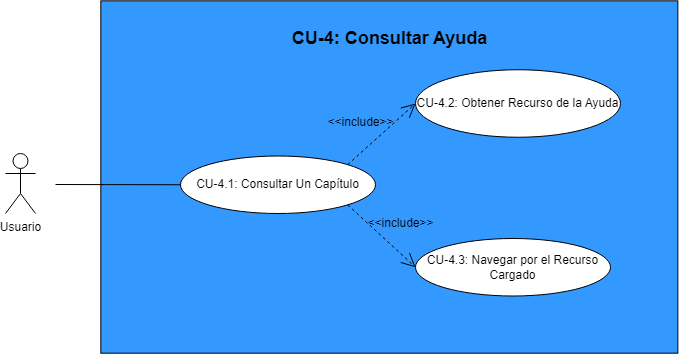
\includegraphics[scale=0.55]{figuras/Cap7/CU4.png}
 	\caption{CU-4: Consultar Ayuda}
 	\label{fig:CU4}
       \end{center}
   \end{figure}

 La especificación del caso de uso se muestra en la tabla \ref{tabla714}.

 \begin{longtable}[H]{|>{\columncolor[rgb]{0.63,0.79,0.95}}m{6cm} | m{8.5cm} |}
 \caption{Caso de uso: CU-4. Consultar Ayuda} \\
 \endfirsthead
 \multicolumn{2}{c}
 {{ \tablename\ \thetable{} -- continúa de la página anterior}} \\
 \endhead
 \hline \multicolumn{2}{|r|}{{Continúa en la página siguiente}} \\ \hline
 \endfoot
 \hline
 \endlastfoot
  \hline
  \textbf{Nombre} & \textbf{CU-4. Consulta de la ayuda}. \newline \textbf{Nivel}: 1  \\ \hline
  \textbf{Descripción} & Permite al usuario consultar la ayuda de la aplicación.\\ \hline
  \textbf{Actores} & Usuario \\ \hline
  \textbf{Casos de uso} & 
     \begin{enumerate}
     \item \textbf{CU-4.1. Consultar un capítulo}: permite \textit{consultar} un capítulo de la ayuda.
     \item \textbf{CU-4.2. Obtener recurso de la ayuda}: permite \textit{obtener} un capítulo de la ayuda.
     \item \textbf{CU-4.3. Navegar por el recurso seleccionado}: permite \textit{navegar} por un capítulo de la ayuda.
     \end{enumerate} \\ \hline
                                 
  \textbf{Flujo de eventos principal} & 
     \begin{enumerate}
     \item Se \textit{obtiene} un recurso de la ayuda (especificado por el usuario).
     \item El usuario \textit{navega} por el recurso.
     \item El usuario \textit{accede} a otro recurso a través del enlace (para lo que se vuelve al paso 1), o sigue navegando por el mismo.
     \end{enumerate}\\ \hline
                     
  \textbf{Flujo de eventos alternativo} & Si se produce algún error al \textit{cargar} o \textit{navegar} por un recurso de la ayuda, se informa al usuario y se restablece el recurso previo (cerrando la ayuda en caso de que se produzca un fallo).
   \label{tabla714}
 \end{longtable}

Nótese que lo que aquí se llama \textit{recurso} de la ayuda (al igual que sucedió con el tutorial), es realmente un \textit{capítulo} de la ayuda. El hecho de de nominarlo recurso implica que el fichero en cuestión (un recurso del simulador) es buscado y cargado, y por tanto, contiene un capítulo de la ayuda.

Al igual que en el caso de uso anterior, no es necesario un refinamiento más profundo, ya que es una tarea sencilla de implementar y que no supone una mayor complejidad.

 \section{Validación de los casos de uso }

Para asegurar que los casos de uso cumplen con los requisitos funcionales establecidos en el capítulo anterior, se llevará a cabo una validación exhaustiva. Esta validación garantizará que los casos de caso de uso se corresponden adecuadamente con los requisitos del sistema y funcionan de manera esperada en distintos escenarios.

% El proceso de validación consistirá en revisar cada caso de uso y verificar que todos los pasos y alternativas responden a los requisitos funcionales descritos. Se documentarán cualquier discrepancia o área de mejora, asegurando que el sistema final sea robusto y cumpla con las expectativas de los usuarios.

% Los resultados de la validación se presentarán en un informe detallado que incluirá tanto las conformidades como las no conformidades identificadas durante el proceso. Este informe servirá como guía para las futuras fases de desarrollo y refinamiento del sistema.

% De esta manera, se garantiza que el sistema no solo cumple con los requisitos establecidos, sino que también es eficiente y efectivo en su funcionamiento, proporcionando una experiencia satisfactoria para los usuarios.
%%%%%%%%%

 \subsection{Validación del Módulo de Edición de Gramática}

 La primera validación que se realizará será del módulo de edición respecto a los requisitos funcionales del sistema. El resultado de esta validación se recoge en la tabla \ref{val1}.

 \begin{table}[H]
 \begin{center}

  \caption{Matriz de correspondencia RF-Casos de uso}
 
 \resizebox{17cm}{!} {
 \begin{tabular}[c]{| c | c | c | c | c | c | c |c |c |c |c |c |c |c |c |}
 \hline

   \multicolumn{15}{|c|}{\textbf{Casos de uso}} \\ \hline
   \multirow{15}{0.3cm}{\begin{sideways}\textbf{Requisitos funcionales  \ \ \ \ \ \ \ \ \ \ \ \ \ \ \ }\end{sideways}} 
  
  & & CU-1.1 & CU-1.2 & CU-1.3 & CU-1.4 & CU-1.5 & CU-1.6 & CU-1.7 & CU-1.8 & CU-1.9 & CU-1.10 & CU-1.11 & CU-1.12 & CU-1.13\\ 
  \cline{2-15}
  &RF-E-1 & X &  & & & & & & & & & & &   \\ 
  \cline{2-15}
  &RF-E-2 & X & X & & & & & & & & & & &  \\ 
  \cline{2-15}
  &RF-E-3 &  &  & X& & & & & & & & & &  \\ 
  \cline{2-15}
  &RF-E-4 &  &  & X & & & & & & & & & &  \\ 
  \cline{2-15}
  &RF-E-5 &  &  & X & & & & & & & & & &  \\ 
  \cline{2-15}
   &RF-E-6 &  &  &  & X& & & & & & & & &  \\ 
  \cline{2-15}
   &RF-E-7 &  &  & & & & &X & & & & & &  \\ 
  \cline{2-15}
   &RF-E-8 &  &  & & & & & & & & & &X &  \\ 
  \cline{2-15}
   &RF-E-9 &  &  & & & & & & & X& & & &  \\ 
  \cline{2-15}
   &RF-E-10 &  &  & & & X& & & & & & & &  \\ 
  \cline{2-15}
   &RF-E-11 &  &  & & & & & X& & & & & &  \\ 
  \cline{2-15}
   &RF-E-12 &  &  & & & & X& & & & &X & & \\ 
  \cline{2-15}
   &RF-E-13 &  &  & & & & & & X& & & & & \\ 
  \cline{2-15}
   &RF-E-14 &  & & & & & & &X & & & & & X \\ 
  \cline{2-15}
   &RF-E-15 &  &  & & & & & & & &X & & &  \\ \hline

 \end{tabular}
 }
  \label{val1}
  \end{center}
 \end{table}

\newpage

 \subsection{Validación del Módulo de Simulación de Gramática}

 La segunda validación que se realizará será del módulo de simulación respecto a los requisitos funcionales del sistema. El resultado de esta validación se recoge en la tabla \ref{val2}.

 \begin{table}[H]
 \begin{center}

  \caption{Matriz de correspondencia RF-Casos de uso}
 
 %\resizebox{17cm}{!} { QUITADO
 \begin{tabular}[c]{| c | c | c | c | c | c | c |c |c |}
 \hline

   \multicolumn{9}{|c|}{\textbf{Casos de uso}} \\ \hline
   \multirow{10}{0.3cm}{\begin{sideways}\textbf{Requisitos funcionales  \ \ \ \ \ \ \ \ \ \ \ \ \ \ \ }\end{sideways}} 
  
  & & CU-2.1 & CU-2.2 & CU-2.3 & CU-2.4 & CU-2.5 & CU-2.6 & CU-2.7 \\ 
  \cline{2-9}
  &RF-S-1 & X & X & & & & &    \\ 
  \cline{2-9}
  &RF-S-2 & X & X & & & & &    \\ 
  \cline{2-9}
  &RF-S-3 &  &  & &X & & &     \\ 
  \cline{2-9}
  &RF-S-4 &  &  & &X & & &    \\ 
  \cline{2-9}
  &RF-S-5 &  &  & & X& & &     \\ 
  \cline{2-9}
   &RF-S-6 &  &  & &X & & &    \\ 
  \cline{2-9}
   &RF-S-7  &  &  & & & X& &    \\ 
  \cline{2-9}
   &RF-S-8  &  &  & & &X & &    \\ 
  \cline{2-9}
   &RF-S-9 &  &  & & & &X &    \\ 
  \cline{2-9}
   &RF-S-10 &  &  & & & &X &    \\ 
  \cline{2-9}
   &RF-S-11 &  &  & & & &X &     \\ 
  \cline{2-9}
   &RF-S-12 &  &  & & & & &X   \\ 
  \cline{2-9}
   &RF-S-13 &  &  & &X & & &    \\ 
  \cline{2-9}
   &RF-S-14 &  &  & & & & &X    \\ 
  \cline{2-9}
   &RF-S-15 &  &  & & & & & X   \\
   \cline{2-9}
   &RF-S-16 &  &  & X& & & &X    \\ 
   \cline{2-9}
   &RF-S-17 &  &  & & & & &X    \\ 
  \cline{2-9}
   &RF-S-18 &  &  & & & & & X   \\ \hline
 \end{tabular}
 %} QUUITADO
  \label{val2}
  \end{center}
 \end{table}


 \subsection{Validación del Módulo del Tutorial}

 La matriz de validación de este Módulo se recoge en la tabla \ref{val3}.

 \begin{table}[H]
 \begin{center}

  \caption{Matriz de correspondencia RF-CU, Módulo tutorial}
 
 %\resizebox{7cm}{!} {
 \begin{tabular}[c]{| c | c | c | c | c | }
 \hline

   \multicolumn{5}{|c|}{\textbf{Casos de uso}} \\ \hline
   \multirow{4}{0.3cm}{\begin{sideways}\textbf{R. funcionales}\end{sideways}} 
  
  & & CU-3.1 & CU-3.2 & CU-3.3 \\ 
  \cline{2-5}
  &RF-T-1 & X &  &   \\ 
  \cline{2-5}
  &RF-T-2 &  & X & X  \\
  \cline{2-5}
  &RF-T-3 &  & X &   \\    \hline

 \end{tabular}
 %}
  \label{val3}
  \end{center}
 \end{table}

 \subsection{Validación del Módulo de la Ayuda}

 La matriz de validación de este Módulo se recoge en la tabla \ref{val4}.

 \begin{table}[H]
 \begin{center}

  \caption{Matriz de correspondencia RF-CU, Módulo ayuda}
 
 %\resizebox{7cm}{!} {
 \begin{tabular}[c]{| c | c | c | c | c | }
 \hline

   \multicolumn{5}{|c|}{\textbf{Casos de uso}} \\ \hline
   \multirow{5}{0.3cm}{\begin{sideways}\textbf{R.  funcionales}\end{sideways}} 
  
  & & CU-4.1 & CU-4.2 & CU-4.3 \\ 
  \cline{2-5}
  &RF-A-1 & X &  &   \\ 
  \cline{2-5}
  &RF-A-2 &  & X & X  \\
  \cline{2-5}
  &RF-A-3 &  & X &   \\\hline

 \end{tabular}
 %}
  \label{val4}
  \end{center}
 \end{table}